%%%% CAPÍTULO 1 - INTRODUÇÃO
%%
%% Deve apresentar uma visão global da pesquisa, incluindo: breve histórico, importância e justificativa da escolha do tema,
%% delimitações do assunto, formulação de hipóteses e objetivos da pesquisa e estrutura do trabalho.

%% Título e rótulo de capítulo (rótulos não devem conter caracteres especiais, acentuados ou cedilha)

\chapter{Introdução}\label{cap:introducao}

Neste capítulo, procura-se lançar o tema da pesquisa, fundamentado na necessidade de compreender e avaliar os níveis de maturidade das organizações frente aos paradigmas da Indústria 5.0, por meio da aplicação da Lógica Paraconsistente como ferramenta de apoio à tomada de decisão em contextos de incerteza e contradição.

\section{Tema}

As transformações industriais ao longo da história moldaram a estrutura produtiva da sociedade.
A Primeira Revolução Industrial, foi impulsionada pela energia a vapor, marcando a transição da produção manual para o modelo fabril mecanizado.
Em seguida, a Segunda Revolução Industrial, trouxe a eletricidade e a produção em massa, elevando a produtividade drasticamente.
Mais recentemente, a Terceira Revolução Industrial integrou eletrônica, automação e tecnologias da informação e comunicação, levando à produção automatizada.
Nas últimas décadas, a Quarta Revolução Industrial, ou Indústria 4.0, focou na interconectividade de sistemas físicos e digitais, utilizando tecnologias como \gls{IoT} e computação em nuvem e inteligência artificial.
Essa fase da revolução industrial buscou automação avançada, decisões autônomas e customização em massa \cite{VALETTE2023}.
Contudo, a Indústria 4.0 foi criticada por sua abordagem predominantemente tecnológica, negligenciando aspectos humanos, sociais e ambientais dos sistemas produtivos.
Essa falha na aboradagem abriu caminho para o surgimento da Indústria 5.0, que busca reintroduzir valores como a centralidade humana, a sustentabilidade e a resiliência \cite{Xu2021, PIZON2023}.

Por isso, a Indústria 5.0 representa a evolução do paradigma da Indústria 4.0, estendendo o foco exclusivo na automação e eficiência operacional para integrar dimensões socioeconômicas.
Esse novo paradigma industrial prioriza a colaboração entre humanos e máquinas e está centrada na busca da valorização da criatividade humana.
Dessa forma, desenvolvendo ambientes de trabalho mais saudáveis, estimulando o trabalho criativo e colaborativo, bem como integrando valores éticos e sociais aos processos industriais.
Os outros pilares da Indústria 5.0 incluem sustentabilidade e resiliência utilizando a tecnologia como meio de ampliar as capacidades humanas.
% \cite{euCommission2021,Xu2021}.

O conceito "Indústria 5.0" ganhou destaque em documentos estratégicos da União Européia desenvolvidos por \citeonline{euCommission2021}, que enfatizam a necessidade de sistemas industriais resilientes, sustentáveis e centrados nas pessoas.
Essa mudança de modelo industrial reflete o reconhecimento de que desafios contemporâneos, como mudanças climáticas, envelhecimento populacional e escassez de recursos, exigem um modelo de produção mais sensível às necessidades humanas e ambientais.

A proposta da Indústria 5.0 envolve um redesenho do sistema produtivo, no qual a tecnologia é utilizada como meio para potencializar as capacidades humanas, promovendo um ambiente de produção que integre valores éticos às operações industriais.
Esse novo paradigma industrial representa uma aboradagem hoslística que demanda transformações organizacionais profundas, deslocando o foco exclusivo da produtividade para a criação de valor social. % \cite{HeinPensel2023}

Nesse contexto, torna-se necessário avaliar em que medida as organizações estão prontas para essa transformação.
A mensuração do grau de maturidade organizacional frente à Indústria 5.0 possibilita identificar lacunas estruturais, definir diretrizes de transformação e orientar políticas industriais.
A maioria dos modelos de avaliação de maturidade existentes ainda se fundamenta nas premissas da Indústria 4.0, priorizando a maturidade tecnológica e negligenciando dimensões como sustentabilidade e ética digital \cite{Lucato2019,HeinPensel2023}.
Assim, surge a necessidade de instrumentos mais aderentes à realidade da Indústria 5.0.
\citeonline{HeinPensel2023} realizaram uma revisão sistemática da literatura e identificaram que, embora existam diversos modelos de maturidade voltados à Indústria 4.0, a maioria negligencia os pilares essenciais como bem-estar dos trabalhadores, inclusão social e responsabilidade ambiental.
Por isso, a avaliação de maturidade nesse novo cenário apresenta desafios como a ausência de modelos consolidados, critérios qualitativos subjetivos e a coexistência com elementos contraditórios.

Além disso, o modelo proposto por \citeonline{BARO2025}, fundamentado na Teoria Sociotécnica desenvolvida por \citeonline{Trist1981}, representa um avanço ao integrar quatro perspectivas interdependentes: estratégia sistêmica, sustentabilidade, centralidade no ser humano e resiliência.
Essa abordagem oferece a granularidade necessária para traduzir os princípios de alto nível da Indústria 5.0 e da Teoria Sociotécnica em um modelo estruturado e permite que as organizações avaliem seu estado atual de implementação da Indústria 5.0 e alinhem suas estratégias com suas capacidades, recursos e objetivos atuais.
Além disso, os autores destacam a escassez de modelos práticos e a necessidade de desenvolvimento de ferramentas de diagnóstico que considerem os fatores humanos e sociais como fatores essenciais do processo de avaliação de maturidade.

Um instrumento diagnóstico capaz de representar e processar informações contraditórias, permitindo, assim, capturar a complexidade sociológica desse novo paradigma industrial, pode ser representado pela Lógica Paraconsistente.
Esta aboradagem lógica permite a tomada de decisões mesmo diante de inconsistências ou dados conlfitantes.Existem aplicações da lógica paraconsistente /TODO em sistemas de controle, inteligência artificial e diagnósticos, especialmente na área médica, demonstram sua robustez frente a incertezas e contradições \cite{SilvaFilho1999, CarvalhoBrunsteinAbe2003, CarvalhoJunior2024}.

\caixa{TO DO}{Ler dissertação do professor para inspiração em relação ao uso de citações diretas}
 
\caixa{TO DO}{Tratar do encadeamento dos assuntos no subtítulo Tema}


\section{Delimitação do Tema}

A presente pesquisa concentra-se no desenvolvimento de um instrumento diagnóstico para a avaliação de maturidade da Indústria 5.0, com um recorte metodológico específico na aplicação da \gls{LPA2v}.
O escopo do trabalho abrange a definição dos critérios de avaliação alinhados aos pilares da Indústria 5.0, a estruturação de um algoritmo de análise baseado na \gls{LPA2v} e o desenvolvimento de um instrumento diagnóstico.
Restringir a metodologia ao uso da \gls{LPA2v}, visa explorar sua capacidade de representar critérios muitas vezes subjetivos ou contraditórios, como bem-estar dos trabalhadores ou equilíbrio entre automação e autonomia humana.
Diversos estudos mostram que os modelos de maturidade atuais, mesmo os que começam a considerar a Indústria 5.0, ainda carecem de instrumentos formais capazes de lidar com a complexidade socio-técnica desse novo paradigma \cite{BARO2025, HeinPensel2023}.
Assim, propõe-se investigar a suficiência da \gls{LPA2v} como base para representação e análise da maturidade organizacional em termos dos pilares da Indústria 5.0 como human-centricidade, sustentabilidade e resiliência.

\section{Problema}
\caixa{TO DO}{Ler a seção da dissertação do professor. Lembrando que o problema tem que terminar com a pergunta da pesquisa}

Os instrumentos atualmente disponíveis para avaliação de maturidade organizacional foram concebidos majoritariamente sob a lógica da Indústria 4.0 e permanecem centrados em critérios técnico-operacionais.
Essa lacuna é evidenciada por \citeonline{HeinPensel2023}, que mostram que poucos modelos existentes contemplam dimensões qualitativas cruciais da Indústria 5.0, como bem-estar dos trabalhadores, ética digital e impacto socioambiental.

Neste cenário, a \gls{LPA2v} apresenta-se como uma alternativa formal viável para representar esses estados de evidência conflitante, viabilizando análises diagnósticas mesmo sob condições de incerteza \cite{JoseSilvaFilho2006, CarvalhoBrunsteinAbe2003, CarvalhoJunior2024}.
No entanto, observa-se que ainda não existem modelos específicos de avaliação diagnóstica da maturidade em Indústria 5.0 fundamentados na \gls{LPA2v}.
Dessa forma, discutimos a aplicação da \gls{LPA2v} para desenvolver um instrumento diagnóstico capaz de avaliar os níveis de maturidade de uma organização frente às dimensões da Indústria 5.0.

\section{Objetivos}

\subsection{Objetivo Geral}

Desenvolver um instrumento diagnóstico, utilizando a \gls{LPA2v}, para avaliação dos níveis de maturidade da Indústria 5.0 em organizações industriais.

\subsection{Objetivos Específicos}

\begin{itemize}
  \item Revisar os modelos de avaliação de maturidade existentes tanto para a Indústria 4.0 quanto para indústria 5.0;
  \item Identificar e estruturar os critérios e dimensões relevantes para diagnóstico de maturidade na Indústria 5.0;
  \item Modelar os critérios e dimensões selecionados utilizando a \gls{LPA2v};
  \item Propor um algoritmo para-analisador, baseado em \gls{LPA2v}, capaz de interpretar e classificar os níveis de maturidade.
  \item Aplicar o modelo proposto em um estudo de caso, validando sua capacidade de gerar diagnósticos sob condições de incerteza e contradição;
\end{itemize}

\section{Justificativa}

Como a \gls{LPA2v} é capaz  de lidar formalmente com incertezas e contradições, o modelo proposto busca suprir uma lacuna metodológica e atender à demanda por ferramentas avaliativas mais alinhadas aos novos princípios industriais.
A contribuição esperada é tanto teórica, expandindo o campo de aplicação da \gls{LPA2v}, quanto prática, ao oferecer um modelo aplicável em contextos organizacionais reais que buscam se alinhar às diretrizes da emergente Indústria 5.0.

\section{Metodologia}

A metodologia proposta neste trabalho está organizada em quatro etapas principais:
\begin{enumerate}[label=\roman*.]
    \item Revisão da literatura e definição das dimensões de análise
    \item Estruturação do modelo avaliativo utilizando a \gls{LPA2v}
    \item Aplicação do modelo em uma organização industrial
    \item Avaliação dos resultados e da aplicabilidade do modelo proposto
\end{enumerate}

Na primeira etapa, será realizada uma revisão sistemática da literatura com o objetivo de identificar os critérios qualitativos relevantes para compor um diagnóstico de maturidade voltado à Indústria 5.0.
Serão consideradas dimensões alinhadas aos pilares desse novo paradigma, como centralidade no ser humano, sustentabilidade, ética digital e resiliência organizacional \cite{euCommission2021}.

Com base nas dimensões identificadas, será estruturado um conjunto de fatores de influência, que representam as principais variáveis intervenientes na determinação do nível de maturidade.
Esses fatores serão organizados em seções em que cada uma corresponde a um domínio conceitual da Indústria 5.0. 

Em seguida, o modelo será aplicado a partir de avaliações realizadas por especialistas do contexto analisado, os quais atribuirão, para cada fator, os pesos relativos e os graus de evidência favorável ($\mu_1$) e desfavorável ($\mu_2$).
Após a coleta dos dados e definição do nível de exigência, os resultados obtidos serão interpretados considerando os graus de certeza e contradição. Por fim, avalia-se a capacidade do modelo em produzir diagnósticos consistentes.

\section{Estrutura do Trabalho}

Este trabalho está organizado em cinco capítulos, conforme descrito a seguir:

\begin{itemize}
    \item \textbf{Capítulo 1- Introdução}: Apresenta o tema de estudo, sua delimitação do tema, o problema de pesquisa, os objetivos geral e específicos, a justificativa, a metodologia adotada e a estrutura geral da pesquisa acadêmica.
    
    \item \textbf{Capítulo 2 - Indústria 5.0}: Trata da fundamentação teórica sobre a Indústria 5.0, destacando seus pilares conceituais e a necessidade de abordagens diagnósticas mais alinhadas a esse novo paradigma.
    
    \item \textbf{Capítulo 3 - Lógica Paraconsistente}: Apresenta a \gls{LPA2v}, incluindo a metodologia a ser utilizada para avaliação diagnóstica.
    
    \item \textbf{Capítulo 4 - Modelo de Avaliação Diagnóstica}: Propõe a aplicação e análise do método paraconsistente de decisão para avaliação diagnóstica de maturidade organizacional frente à Indústria 5.0.
    Este capítulo descreve a criação do modelo, os fatores de influência utilizados, a análise dos resultados obtidos após a aplicação do modelo.
    
    \item \textbf{Capítulo 5 - Conclusões e Considerações finais}: Apresenta as considerações finais do trabalho as limitações da abordagem desenvolvida e sugestões para estudos futuros que possam aprimorar ou expandir o modelo proposto.
\end{itemize}

\begin{comment}
\noindent Exemplos de citação:

Segundo \citeonline{Coulouris2013}.

Segundo \citeonline[p. 40]{Coulouris2013}.

Citação no final do Parágrafo~\cite{Coulouris2013}. 

Citação no final do Parágrafo com número de página~\cite[p. 40]{Coulouris2013}.

%(Modelo de referência: pessoa jurídica)
Citação no final do Parágrafo~\cite{NBR6023:2018}

%(Modelo de referência: pessoa jurídica)
Citação no final do Parágrafo~\cite{NBR6027:2012}

%(Modelo de referência: pessoa jurídica)
Citação no final do Parágrafo~\cite{NBR6028:2021}

Segundo a \citeonline{NBR14724:2011}.

Citação no final do Parágrafo~\cite{NBR10520:2002}

Citação no final do Parágrafo~\cite{NBR14724:2011}.

% (Modelo de referência de trabalho acadêmico).
Citação no final do Parágrafo~\cite{Andrade2005}

% (Modelo de referência: capítulo de livro).
Citação no final do Parágrafo~\cite{Borges2014}

% (Modelo de referência: leis, decretos, portarias, etc.)
Citação no final do Parágrafo~\cite{BRASIL:1998}

% (Modelo de referência: livro com subtítulo). Nome com sufixo "Von" - Configuração no bib
Citação no final do Parágrafo~\cite[p. 66]{KROGH:2001}

Citação no final do Parágrafo~\cite{Faina2001}

% (Modelo de referência: livro com subtítulo).
Citação no final do Parágrafo~\cite{Davenport2012}

% (Modelo de referência: artigo de periódico).
Citação no final do Parágrafo~\cite{Monteiro2009}

%(Modelo de referência: artigo de periódico). Nome familiar "Junior"
Citação no final do Parágrafo~\cite{Sanches2024}

% (Modelo de referência: trabalho publicado em evento).
Citação no final do Parágrafo~\cite{Renaux2001}

Em relação ao assunto, o apresentado nesta seção pode estar relacionado a trabalhos de outros autores ou ao assunto que fornece a fundamentação (motivação) para o trabalho a ser desenvolvido. Se o assunto está relacionado a trabalhos de outros autores, a contribuição do trabalho é definida em relação ao que já foi pesquisado nesse assunto. Se o assunto será utilizado para embasamento do que será proposto, explicitar como o trabalho se insere nesse assunto. A contribuição pode, ainda, estar relacionada a uma necessidade de mercado ou a uma oportunidade decorrente de algum problema real para o qual se pretender propor uma solução. Nesse caso, o assunto fornece um contexto teórico de suporte para o problema e/ou a solução.

O importante nesta seção é deixar claro do que se trata o trabalho (assunto ou tema), identificar o objeto de pesquisa, como será encaminhada a solução (procedimento metodológico, tecnologias, ferramentas utilizadas) e o que se pretende ao final do trabalho, sem explicitar a solução e os resultados.



\begin{photograph}[!htb]%% Ambiente figure
    %\captionsetup{width=0.55\textwidth}%% Largura da legenda
    \caption{Exemplo de fotografia}%% Legenda
    \label{fig:exemplo1}%% Rótulo
    
\includegraphics[scale=0.4]{foto1}%% Dimensões e localização
    \fonte{Autoria Própria}%% Fonte
    \addcontentsline{loge}{photograph}{\protect\numberline{\thephotograph}Exemplo de fotografia.} % Adiciona à lista de ilustrações
\end{photograph}

Os objetivos específicos são opcionais, ou seja, somente devem ser apresentados se caracterizarem resultados parciais gerados a partir do objetivo geral, os quais sejam considerados úteis para a comunidade acadêmica, para a sociedade ou para o ambiente profissional. Uma observação importante é que os resultados sejam passíveis de comprovação, ou seja, se o objetivo for: “Oferecer agilidade e confiabilidade aos processos gerenciais da empresa”, significa que o trabalho deverá realizar testes com relação a esses atributos, cujos resultados deverão ser apresentados nas discussões do trabalho.

\begin{graph}[!htb]%% Ambiente figure
    %\captionsetup{width=0.55\textwidth}%% Largura da legenda
    \caption{Exemplo de gráfico}%% Legenda
    \label{graph1}%% Rótulo
    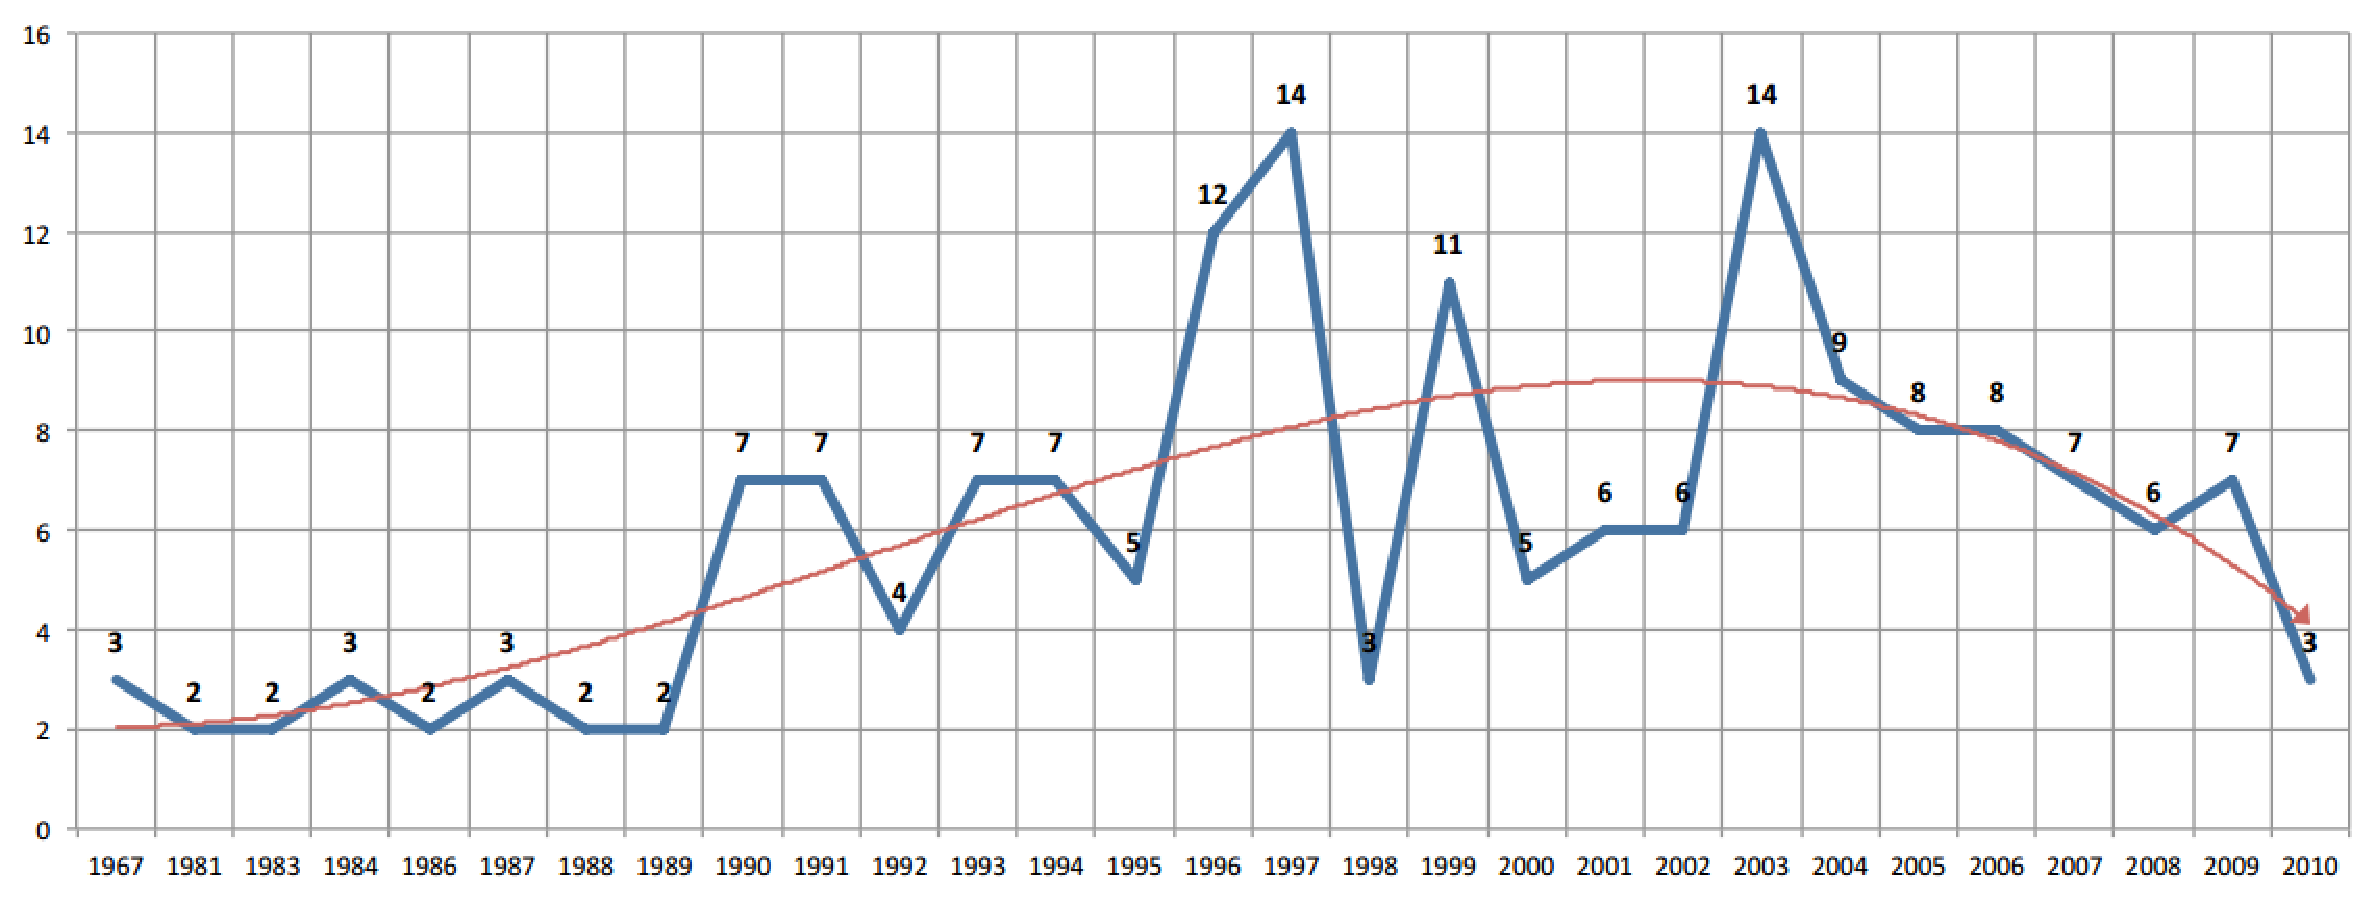
\includegraphics[scale=0.4]{grafico2}%% Dimensões e localização
    \fonte{Adaptado de \citeonline[p.~4]{UTFPR2008}}%% Fonte
    \addcontentsline{loge}{graph}{\protect\numberline{\thegraph}Exemplo de gráfico.}
\end{graph}


Destaca-se que os objetivos específicos não incluem as etapas do processo de desenvolvimento de software (realizar a modelagem, a análise, o projeto...) ou outras atividades necessárias para alcançar o objetivo geral, como, estudar as tecnologias necessárias para modelagem e implementação do sistema. Dentre as exceções estão a realização de estudos, procedimentos, métodos e técnicas considerados inéditos e de relevância para outros trabalhos a serem realizados na mesma área. Contudo, o resultado deste estudo deve ser documentado de forma que seja conhecimento disponibilizado para quem lê o trabalho.


\subsection{Seção ternária (sublinhado)}

xxxxxxxx mkmdasda

asdadas

 
\subsubsection{Seção quaternária (sublinhado)}

xxxxxxxxx

dasda

\subsubsubsection{Seção quinária (itálico)}
\end{comment}
\begin{comment}
Justificar o objeto de pesquisa (o que será feito) e a forma de resolução do problema (como fazer). A forma de resolução pode estar centrada no método, nas tecnologias, no uso de conceitos (fundamentação teórica).

A Justificativa explicita porque desenvolver o referido trabalho, como o mesmo se insere no contexto de pesquisa, de produção científica. Pode incluir o porquê utilizar as tecnologias e ferramentas indicadas, a contribuição em termos de inovação ou mesmo de aprendizado.

O trabalho não precisa ser justificado em decorrência de ser inovador ou por ter gerado uma significativa contribuição ao conhecimento na área em que o mesmo se insere. Pode referir-se simplesmente à aplicabilidade de conhecimentos adquiridos durante o curso. Sendo assim, a justificativa não deve ser elaborada considerando um mercado a ser atingido e sim com relação ao uso de tecnologias aprendidas e/ou estudadas, o conhecimento e aprendizado do aluno e a aplicabilidade do trabalho desenvolvido.
\end{comment}
\begin{comment}
A estrutura do trabalho contém uma relação dos capítulos e uma descrição sucinta do que cada um deles contém. Esta seção fornece uma visão geral do trabalho no sentido da sua estrutura em capítulos\footnote{Teste de nota de rodapé 2.}.

\caixa{Atenção}{O OverLeaf está demorando muito para compilar o modelo com o Capítulo de Exemplos, que explica como usar o LaTeX. Assim, esse capítulo foi removido (está comentado para não compilar), mas há um arquivo chamado \texttt{exemploPDF.pdf}, na raiz do projeto, que contém esse capítulo de exemplos!}
\end{comment}






